El siguiente gráfico de barras muestra el número de alumnos matriculados en una facultad por año de estudios, correspondientes a los años 2015 a 2018.

\centerline{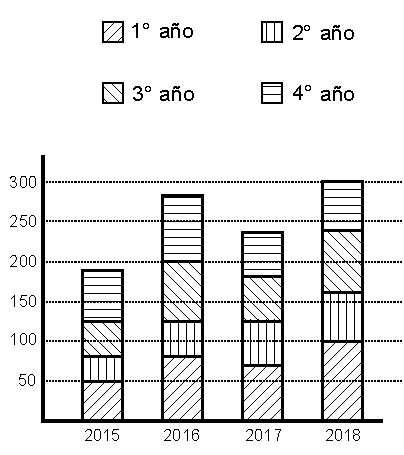
\includegraphics[width=6cm]{figura}}

Luego de estudiar atentamente el gráfico señale la alternativa que presente la secuencia correcta, después de determinar si la proposición es verdadera (V) o falsa (F).
\begin{enumerate}[I.]
\item El número de alumnos en el tercer año de estudios, del año 2018 fue 80.
\item En 2015 los alumnos matriculados en el primer y segundo año representan el 40\% de los alumnos matriculados.
\item Los alumnos de 2\textordmasculine\ año experimentan un menor crecimiento en porcentaje del año 2015 al año 2016 comparado con el incremento entre 2017 y 2018.
\end{enumerate}
\ctdt{VFF}{VVF}{FFV}{VVV}{FVF}